
%\chapter{Objectives}

\chapter{Context}

\section{Global change: how to describe the future of alpine ecosystems}

\subsection{The value of ecosystems}

\paragraph{New logic}
Everyone has a particular relationship with nature. The vision we put behind this word depends on the way we experienced nature, it can be temperate or tropical forest, mountain rivers or cliffs on the ocean littoral, bird songs or wind between stones. Anybody that shares one of these visions, I am sure wants to preserve natural systems. But facing this emotional perception and inner desire to see these ecosystems be preserved, other forces pushes in other directions. The reduction of biodiversity is increasing at dangerous rates, the deforestation threaten the largest forest systems, insects are less and less presents and animals are repelled to fragmented and diminishing habitats. Other logics than emotional attachment and will to protect impact all natural systems around the world. To be protected, the natural systems needed a way to be integrated in these logics, and the notion of \textemph{ecosystem services} was developed by \cite{costanza_value_1997}. This notion encompass all benefits human extract from ecosystems. It enables a categorisation of services and their quantification (that can go to the monetisation), and therefore allow them to be taken into consideration in global logic of capital, investment and value.


\paragraph{Services}
But, what is the value of an ecosystem?

If ones could be tempted to answer that the value of an ecosystem cannot be measure, it is are to deny that all ecosystems do not benefit to human in the same way. Face to the diversity of ecosystems and services they provide, we can try to develop a short answer for the object of study to this document: mountain grasslands.

\textemph{Mountain grasslands} designs in this document all grasslands, below and above the treeline, that have short growing seasons delimited by snow covered periods and experience high variations in temperature and water availability. This term is intentionally generic as the scope of this work is relatively broad and theoretical.

Mountain grasslands provide numerous services, that can be divided in multiple categories such as provision, cultural and regulating services. Provision services are related to the quantity and quality of primary resources the grasslands provide. Fodder production and quality are the main measures of provision services. Other services can be included in this category: diversity of flowers and phenology for flower production for instance. Productivity is also interesting to assess carbon capture, a regulating service. Soil nutrient availability and water filtering are other regulating services impacted by the identity and diversity of species populating mountain grasslands. Finally, cultural services, related to tourism activity and landscape appeal are also related to grasslands species diversity.

The ecosystem services are tightly related to ecosystem properties (ass illustrated in figures \ref{fig:preporties}), that can be extracted from the description of the grassland communities. But grasslands community are natural systems driven by environmental variables, and these drivers are changing.

\subsection{Global change}

Mountain grasslands are maintained by strong climatic constraints that limit growth rate and lifeforms  \parencite{koorner_alpine_2003}, but also frequent grazing or cutting perturbation regimes that strongly limit the growth woody species and favour low stature species or rapid growth herbs \parencite{diaz_plant_2007}. But these drivers are changing at alarming rates and mountain grasslands are suspected to be very vulnerable \parencite{engler_21st_2011} due to higher variations in water availability regimes, stronger isolation (island effect due to rise in temperature) and reduction of the grazing pressure.

\paragraph{Climate change}
Rising temperatures due to anthropogenic greenhouse gases has a strong effect on mountain climate. 


\paragraph{Effect of management}

trade-off lavorel and \parencite{schirpke_multiple_2012}

management change the position along these trade-off

climate also change things


\subsection{Properties and services}

\subsection{The need for mechanistic models}

\paragraph{A new world}
outside what's known, extrapolations and experimentations

The combined effect of land-use mutations and climate changes will lead to environmental conditions never experienced by such systems. Predicting the future in new conditions implies extrapolating multiple effects not tested in combination: with cumulative effects and potential synergies (carbon dioxide increase and grazing abandonment) or effects balancing each others (grazing abandonment and higher frequency drought events).


 \paragraph{Complexity}
 this title is not helpful -
 
 combined effects
 
 community responses: different processes (recruitment, growth, plasticity etc...) & levels (indiv, pop, metacommunity)
 

 In addition to complexity of combined effects of global change drivers, complexity is inherited from the complexity of the community dynamics. Interacting species may change response of the system, and should be better taken into accounts \parencite{gilman_framework_2010}. To answer this challenge, large scale experiments are conduced such as Cedar Creek experiment in the United-States, or JENA experiment in Germany. These experiments give high value experimental data for various conditions and a variety of species, where interactions can be studied as well as management effects.
 Transplant experiments are also conduced to investigate the effects of temperature rise on the productivity, diversity and structure of the community. (Need more references) Showing increase in productivity and dicrease in diversity, as well as a shift toward more acquisitive species \parencite{debouk_functional_2015}.
 
 Observed effects: jung, transplant, effect on diversity and productivity.
 
contrasting effects as function of elevation: change in identity (abundance) and increased diversity in low altitude, but decrease in diversity in high altitude \parencite{rosbakh_elevation_2014}
 
 But, temporal effects, history (that guy from ecoveg talk) hysteresis effect, metapop and invasion effects, balance between intra-specific and einter-sp responses...
 
 Modelling approaches   
 
 
limits of empirical studies: \parencite{merila_climate_2014}

 
 \parencite{schirpke_multiple_2012}

 The increasing variability in those conditions 
 
 and uncertainty that would require multiple experiments. Models allow to explore multiple scenarios.
 
%
%\section{Community dynamics: complexity emerging from parts and the role of phenotypic plasticity}
%title too vague to bring meaning, should put both parts together.

\subsection{The limit of classic patterns}

niche vs process: stronger effects because no plasticity or local adaptation \cite{morin_comparing_2009}
\subsection{The rise of individual-based approaches}

LINGRA-CC \cite{rodriguez_lingra-cc:_1999} to test gc effect on productivity : higher productivity allowing shorter intervals between cutting




\subsection{When phenotypic plasticity makes things complicated}

plasticity change response \cite{morin_comparing_2009}

phenotypic changes in competition intensity that increase negative effect \parencite{hanel_phenotypic_2015}

\subsection{Gaps to fill}

scales and processes (climate, management etc...)
put the resoure in the center (fate-hd)

process and mechanisms
\parencite{berger_competition_2008}: effect on local env., adaptive beh, below-ground.

lack of diversity. 

%
%
%
%\section{Global change and community dynamics in alpine grasslands}
%\begin{figure*}
%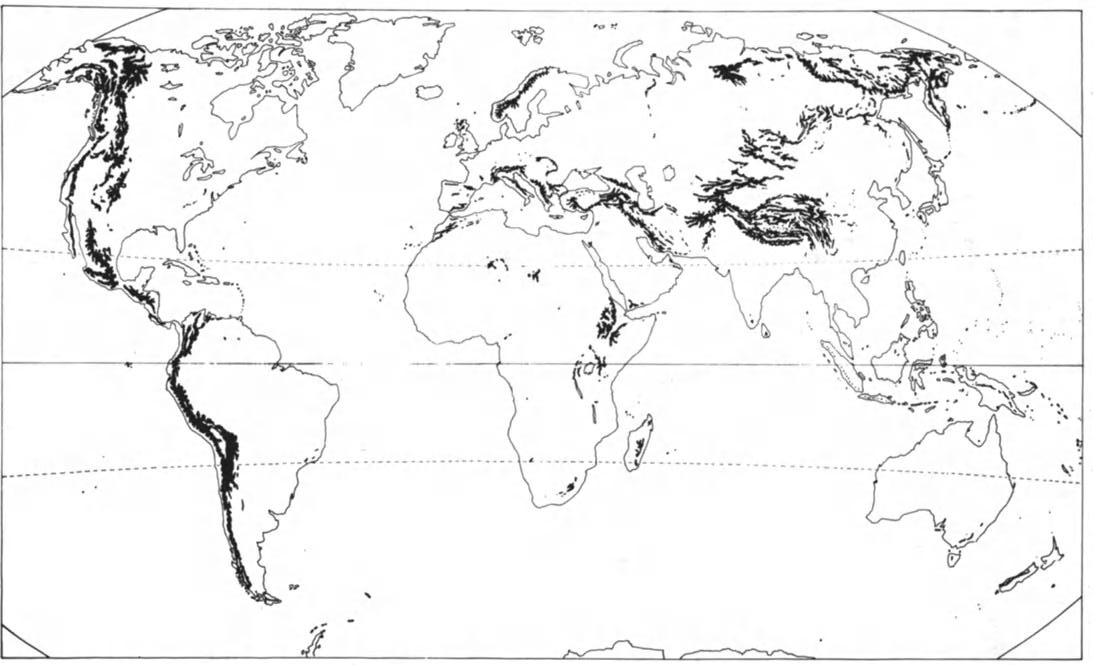
\includegraphics{./1_Introduction/graphics/alpine_distribution.jpeg}
%\caption{Distribution of alpine habitats}
%\end{figure*}
%
%Climate change is probably the greatest challenge the humanity has to face this century. Expected drastic changes in both average climatic conditions and punctual climatic event frequencies and intensities will, and already have, an impact all around the globe on multiple aspects of our lives. From agricultural and economic, to social and political, but also scientific and technical, the problems for human societies are numerous and multidimensional.\\ 
%Need to better understand and predict natural systems. Mountain grasslands are susceptible to be greatly impacted (even if certain think they might not). And in new ways as the rising temperature will certainly lead to migration to higher altitude, increasing the island characteristic of alpine habitats and reducing links between communities, and at the same time increasing the opportunity of invasion by lower altitude higher temperature species.\\
%\indent Detail a bit the characteristic of mountain grasslands, (snow, islands, grazing) the effect on species (snow-bed species, link to meta-community, diversity, species adaptation to frost etc... and how global change may affect that.\\
%\indent Because of that mountain grasslands are rich in species, but also vulnerable, that is why in parallel of predicting climate change, we also need to understand ecological mechanisms under this diversity and how they can be affected by global change \sidenote{section \ref{sec:coexistence}}. A key part in community diversity and in adaptation of communities also lies in the diversity and adaptation of individuals, so we are interested in intra-specific diversity and phenotypic plasticity \sidenote{section\ref{sec:intraspe}}.
%
%
%%Take home message ####################################
%\textbf{There is a need for new tools to predict the response of ecosystems to new climate conditions and management scenarios. These tools should integrate the complexity of such system and the mechanisms underlying the dynamic responses of these communities.}
%
%\section{Empirical results, trait approaches and need for a new kind of model in grasslands}
%
%\subsection{On trait-based approaches}
%
%Holy Graal of ecology\\
%Lavorel, Kraft, Kunstler
%
%\subsection{The importance of intra-specific variability}
%
%Jung
%Leps
%Albert
%Kichenin
%Lavorel (hypothesis of traits bell shape)
%Violle ...
%
%%Take home message ####################################
%\textbf{Trait approaches allow for generalisation and more direct link with processes and services. However they ignore variations and processes at lower levels than the species that are of critical importance for the understanding of community dynamics. A mechanistic approach integrating processes at the individual level and rich community complexity are needed.}
%
%\section{Close a gap in grassland modelling}
%
%%Take home message ####################################
%\textbf{Generalizing models for forest ecosystems and complex individual level models for grasslands coexist, but there is a need for a generalizing model at individual scale for grassland communities.}
%
%\section{Effect of phenotypic plasticity on coexistence and community dynamics}
%
%%Take home message ####################################
%\textbf{Despite empirical and theoretical work, the effects of intra-specific variability and plasticity on community dynamics are not fully disentangled. Understanding the effect of individual variations on plant community is crucial and may greatly alter how we envision the future of these ecosystems.}
%
%%_________________________________________________________________________________
%

\chapter{Aims, Objectives and Overview}


\section{Aims: understanding and prediction}

Global change is probably the biggest challenge humanity has to face at the beginning of this millennium. But while action is needed, it requires understanding, and the multiplicity of environmental drivers impacted by global change, whose effects can synergise or balance themselves, in addition to complex structure and dynamics of natural systems make this understanding hard to build and to summarise.

To go beyond traditional pattern-driven ecology and overcome the difficulty of combined causes leading intricate effects, mechanistic approaches should be priviledge. 

The functioning of individuals living in these communities and the dynamics of the resources should be at the core of the new approaches to better understand the trajectories of the ecosystems.

\textemph{Ecosystem} both living and non living components of a systems binded together by interactions. 
%
%Functioning
%Diversity of : drivers, mechanisms, species and strategies
%Flexibility: structure: genericity, experiments, plasticity

\section{Objectives: a new agent-based model for plant community dynamics} % the why
Traditional empirical approaches of observation and controlled experiments provided valuable information on the functioning of these systems. However, they lack power to understand intricate systems and predict their dynamics, especially in case of uncertain scenarios. 

Modelling approaches must be used to build understanding and predictions of natural ecosystems dynamics driven by changing environmental drivers. These models should include the diversity of drivers as well as the diversity and the intrinsic complexity of these systems.

In order to be compensate long development time and to extend the reach of experimental approaches, models should try to keep generic in structure and flexibility in use, while being specialised thanks to parameters or simple equation changes.

\subsection{Generic framework for multi-species and plastic plant modelling} % the how

In the context of mountain grasslands, showing unique levels of diversity despite strong environmental drivers, species diversity cannot be ignored to predict the response of the community. This diversity must be translated into plant functioning differences leading to diverse niches and possible response. In addition to species level dynamics driven by these differences, intra-specific responses cannot be ignored, and a phenotypic plasticity mechanism is needed.



%trade-off that constrain inter and intra differences in the same way

\subsection{Effect of phenotypic plasticity on plant growth and community dynamics}

Intra-psecific variations are espectic to play an important role in the response of mountain grassland communities to global change. The effects of phenotypic plasticity and other source of variations must be disentangled. Explicit integration of phenotypic plasticity in a plant community model will help identify and understand these effects.

As multiple services derive from the main properties of the vegetation of mountain grasslands, it is crucial to establish how phenotypic plasticity specifically impact these properties. Because these properties depend both on properties of the individuals and the relative abundance and diversity of species, effects on processes at both individual and community scales must be investigated.


\section{Thesis overview}

The rest of this thesis is divided in five chapters. The following chapter \ref{part:literature}, in the form of a literature review, introduces the concepts and knowledges that support the approach developed in later chapters. The chapter \ref{part:model} develops the generic framework for plant functioning and phenotypic plasticity from the concepts established in chapter \ref{part:literature} and further extended. Chapters \ref{part:individuals} and \ref{part:community} present respectively individual and community scale results of simulations made with the developed model \model on the effects of phenotypic plasticity on main plant community properties. Finally, the final chapter discusses the outcomes of this work and present path to follow from the present conclusions. Extensions to develop on the model are also proposed.
